\documentclass{article}
\usepackage{graphicx}
\graphicspath{ {images/} }
\usepackage[utf8]{inputenc}



\title{Hilos a nivel del microprocesador}
\author{Juan Felipe Gutiérrez Sánchez }
\date{Proyecto de investigación - Informática 2}


\begin{document}

\maketitle
\begin{figure}
\centering
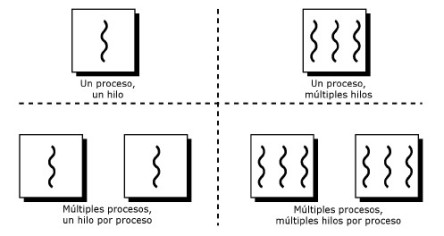
\includegraphics[width=1\textwidth]{foto-3.jpg}
\caption{\label{fig1} Imagen ilustrativa}
\end{figure}


\section{¿Qué es un hilo en el contexto de los microprocesadores?}

Un hilo, es la caracterictica que permite a una aplicacion realizar varias tareas a la vez concurrentemente, los distintos hilos de ejecucion comparten una serie de recursos tales como el espacio de memoria, los archivos abiertos, situacion de autentificacion. Esta accion permite simplificar el diseño de una aplicacion que debe llevar a cabo distintas funciones simultaneamente. [1]

Un ejemplo para entender el concepto seria cuando un servidor web acepta solicitudes de los clientes que piden páginas web. Si este servidor tiene varios clientes y funcionara con un solo hilo de ejecución, solo podría dar servicio a un cliente por vez, y el tiempo que podría esperar un cliente para ser atendido podría ser muy grande. Una posible solución sería que el servidor funcione de tal manera que acepte una solicitud por vez, y que cuando reciba otra solicitud, cree otro proceso para dar servicio a la nueva solicitud. Pero crear un proceso lleva tiempo y utiliza muchos recursos, entonces, si cada proceso realizará las mismas tareas seria mejor utilizar hilos, generalmente es más eficiente usar un proceso que utilice múltiples hilos (un hilo para escuchar las solicitudes, y cuando llega una solicitud, el lugar de crear otro proceso, se crea otro hilo para procesar la solicitud).

\\[0,5cm]


\section{Historia}
El origen de los hilos no es muy exacto, se tiene una noción de su aparición a mediados del año 1965, con el diseño del OS/360 de IBM mencionada en los comentarios de Dijkstra. El lenguaje PL/I definido por IBM realizaba procesos pesados, tareas que dieron como resultado un hilo, pero se cree que nunca fue implementado debido a falta de proteccion entre de los hilos de control. [2]
\\[0.5cm]

\section{Tipos de hilos}

Existen 2 tipos de hilos [3]:

\begin{itemize}
\item  A nivel de usuario (ULT): la aplicación es quien se encarga de la gestión de los hilos, por lo que para estos no es necesario que el SO ayude en el proceso. Para poder programar estos hilos es necesario hacer uso de alguna librería de hilos. Gracias a estos hilos el usuario tiene permitido realizar planificaciones específicas de ejecución.
\item A nivel de kernel o núcleo (KLT): todo el trabajo es realizado por el núcleo, los crea y los organiza para las tareas a ejecutar. Gracias a este tipo de hilos los procesos se realizan mucho más rápido y se ahorran recursos.
\end{itemize}

\section{Implementación hilos por HARDWARE}
es la que viene por defecto en el microprocesador o el procesador, estos poseen una cantidad de núcleos e hilos que pueden utilizar para la realización de procesos, los hilos que posee la unidad de control son reconocidos por el kernel, es decir, son hilos a nivel de kernel, lo que quiere decir que son limitados, dependen del hardware, por ejemplo si de fábrica se establece que tenga ocho hilos no puede poseer un número mayor de hilos a ocho, pero si puede dejar de utilizar un número menor al establecido de fábrica al momento de realizar la ejecución de un proceso. [4]
\\[0.5cm]

\section{Implementación hilos por SOFTWARE}
En una aplicación ULT pura, todo el trabajo de gestión de hilos lo realiza la aplicación y el núcleo o kernel no es consciente de la existencia de hilos. Es posible programar una aplicación como multihilo mediante una biblioteca de hilos. La misma contiene el código para crear y destruir hilos, intercambiar mensajes y datos entre hilos, para planificar la ejecución de hilos y para salvar y restaurar el contexto de los hilos. 
Todas las operaciones descritas se llevan a cabo en el espacio de usuario de un mismo proceso. El kernel continua planificando el proceso como una unidad y asignándole un único estado (Listo, bloqueado, etc.). [5]

\\[0.5cm]




\section{Fuentes de consulta}

Las siguientes fuentes fueron utilizadas para la consulta:

[1] Hilos. https://edwardlozadaso.wordpress.com/hilos/ 

[2] E. Dijkstra, “The next fifty years,” http://www.cs.utexas.edu/users/EWD/12xx/EWD1243a.html

[3] 5. Hilos. https://www.fing.edu.uy/tecnoinf/mvd/cursos/so/material/teo/so05-hilos.pdf

[4] J. Khoury, “What is the difference between hardware and software threads
and how do they c¸ommunicate¿” 2017. [Online]. https://www.quora.com/
What-is-the-difference-between-hardware-and-software-threads-and-how-do-they-communicate

[5] Usos mas comunes de los hilos. https://sistemasoper2.wordpress.com/2014/10/21/usos-mas-comunes-de-los-hilos/





\end{document}
